%\documentclass{sig-alternate}
%\documentclass[]{sig-alternate-05-2015}
%\documentclass[10pt, conference, compsocconf]{IEEEtran}
\documentclass[10pt, conference]{IEEEtran}
\IEEEoverridecommandlockouts      % enable the \IEEEpubid command for the 'conference' class

\usepackage{amsmath}
\usepackage{amsthm}
\usepackage{accents}
\newcommand*\underdot[1]{%
  \underaccent{\dot}{#1}}
\usepackage{mathtools}
\DeclarePairedDelimiter\ceil{\lceil}{\rceil}
\DeclarePairedDelimiter\floor{\lfloor}{\rfloor}
\usepackage{mathrsfs}
\usepackage{times}
\usepackage{multirow}
\usepackage{enumitem}
\usepackage{epsfig}
\usepackage{subfigure}
\usepackage{amsfonts}
\usepackage{amssymb}
\usepackage{graphicx}
\usepackage{url}
%\usepackage{cite}
\usepackage{psfrag}
\usepackage{array}
\usepackage{comment}
\usepackage{mdwmath} % part of Mark Wooding's powerful
\usepackage{mdwtab}  % tools for math, tables, ...
\usepackage{bm} % for the bold font Greek symbols in math mode
\usepackage{color}
%\usepackage[noend]{algorithmic}
\usepackage[noend]{algpseudocode}
\makeatletter
\usepackage{multirow}
\usepackage{algorithm}
\usepackage{xspace}
%\usepackage{flushend}  <-- Bear, ACM do not like balanced last page
\usepackage{natbib}  % for small reference font size
\def\bibfont{\footnotesize}
\setlength{\bibsep}{0.0pt}

%\usepackage{float}
%\usepackage{natbib}  % for small reference font size
%\def\bibfont{\scriptsize}
%\setlength{\bibsep}{0.0pt}
%\usepackage{enumitem}
%\setlist{nolistsep}

% INFOCOM specific space saving tips from Bo
%\renewcommand{\baselinestretch}{0.990}
% place it after 'documentclass' for shrinking line space. Default is 1. 0.92 is the minimum acceptable by INFOCOM
%\usepackage[left=0.625in,right=0.625in,top=0.75in,bottom=1in]{geometry}
% this sets the margins of the 3 sides. The numbers are the minimum acceptable by INFOCOM

\newtheorem{thm}{Theorem}
\newtheorem{cor}{Corollary}
\newtheorem{lem}{Lemma}
\newtheorem{dfn}{Definition}
\newtheorem{pbm}{Problem}
\newtheorem{claim}{Claim}

%\remove copyright box
%\makeatletter
%\def\@copyrightspace{\relax}
%\makeatother


\begin{document}
\sloppy

\title{
Streaming Scalable Video Sequences with Media-Aware Network Elements Implemented in P4 Programming Language
}

\author{ 
\IEEEauthorblockN{Chao-Wen Chen$^1$, Cheng-Hsin Hsu$^1$}
\vspace{2pt}
\IEEEauthorblockA{$^1$Department of Computer Science, National Tsing Hua University, Taiwan}
}
\maketitle

\begin{abstract}
  We aim to reduce the negative impact of dropping packets inside the Internet. There are three drop logic are considered. (i) tail, (ii) enhancement-layer, and (iii) rate-distortion.
\end{abstract}
\begin{IEEEkeywords}
Scalable video streaming, media-aware network element, software-defined network, rate-distortion optimization
\end{IEEEkeywords}

\section{Motivation} \label{sec:motivation}

In recent years, people are getting used to rely on Over-The-Top (OTT) 
services such as Skype, Facebook, Youtube, Netflix, etc. 
Among these services, video streaming is one of the services which 
consumes the most network resources. Video streaming needs more and more bandwidth because receivers prefer higher video quality than before, and thus incur high traffic amount on the best-effort Internet. Turns out streaming high quality video with less network resources becomes much more important.

{\em Scalable Video Coding (SVC) }is one of solutions for network congestion. Each of the SVC sequences contains a base and multiple enhancement layers. Furthermore, the encoder will encode the discardability into the packetize header. Therefore, We can drop the discardable packets without affecting its decodability in the middle-box of the Internet.The dynamic decisions on which video packets to drop can be sub-optimally done by streaming servers or clients without the global knowledge of the Internet. The better way to approach is through {\em Media-Aware Network Elements (MANEs)}, which are switches with knowledge of packets header. However, changing the normal switches into MANEs is quite difficult and thus not likely to happen. Fortunately, with recent advances in {\em Software-Defined Networking (SDN)} and {\em Network Function Virtualization (NVF)}, network switches are much more programmable, and make collaborative MANEs into reality. 




\begin{comment}
Over-The-Top (OTT) video streaming services, like Apple TV, Netflix, and Hulu,
have become very popular, e.g., the streaming device market is projected to
exceed 25 billion USD by 2024, with a 15\%+ annual growth on unit shipments~\cite{ott_market}. These OTT services offer 4k resolution
video sequences, and thus incur high traffic amount on the
best-effort Internet. {\em Scalable Video Coding (SVC)} is a promising solution
to mitigate such excessive traffic: each scalable video
sequence contains a base and multiple enhancement layers, while higher
enhancement layers can be dropped without affecting its decodability.  
The dynamic
decisions on which video packets to
drop can be sub-optimally done by
streaming servers or clients without the global knowledge on the network.
A better way for making decisions is through {\em
Media-Aware Network Elements (MANEs)}, which are switches that have access to
the video-related packet headers and local network conditions, and thus can
make better decisions. By collaboratively considering multiple OTT video
streams sent across a set of interconnected MANEs, an even higher video
quality level is possible. 

Unfortunately, replacing regular switches with MANEs is quite expensive and therefore less likely to happen.
However, with recent advances in {\em Software-Defined Networking (SDN)} and
{\em Network Function Virtualization (NFV)}, network switches are much more
{\em programmable}, which in turn make collaborative MANEs into a reality. 
A recent market report points out that the
SDN/NFV investments from Internet Service Providers (ISPs) 
are expected to grow at an annual rate of 45\% between 2017 and 2020~\cite{sdn_market}. In
other words, programmable switches are going to be deployed in the Internet
scale, and {\em these switches can be programmed into collaborative MANEs for
optimally streaming scalable video sequences.}


In this work, we prototype the very first MANE in P4 programming
language~\cite{BDGI+14} for scalable video streaming. P4 is designed for
realizing different network protocols (in software) on packet processors that
can forward packets at the line speed. We implement intelligent media-aware
packet drop logics in packet processors of P4 switches, and we connect
multiple P4 switches to an ONOS controller through P4 runtime for a
network of collaborative MANEs. We demonstrate our prototype system using
mininet or a few real P4 switches to show its
practicality. Real scalable video sequences are created and used
in our demonstrations, while several demonstration scenarios are used to
show the merits of our system. 
\end{comment}

\section{Research Problem} \label{sec:Remark Problem}

SVC can help us to reduce network congestions but selecting some proper layer to stream isn't a optimal solution. The network condition would change violently in runtime. Select the packets in middle of Internet would be much better than decide them in the beginning. Nevertheless, regular switches in the Internet can't drop any particular packets. The working logic of them is such easy as store and forward all the packets. The packets will be drop without any remedy in UDP protocol which is the most used protocol in video streaming. In SVC sequence, the higher layer can be decode depends on the lower layer. In other words, forwarding the higher enhancement layer without the lower enhancement layer waste the network resource a lot. 

To solve this problem, we are going to use {\em Programming Protocol-Independent Packet Processors (P4)} ~\cite{BDGI+14} programming language to design a switch to drop some useless packets in the middle of the Internet. P4 is a new describing language with following features. (i) Protocol Independent, (ii) Target Independent, and (iii) Field Reconfigurable. Protocol independent allows us to design any protocol we want to forward the packet, and thus we can add some user-specific field in the header for us to make our decision. Target independent allows us to describe everything from high-performance ASICs to software switches. Field reconfigurable allows us to change the way our switches process packets after we deploy our p4 program. 

\begin{figure}[tbh]
    \centering
    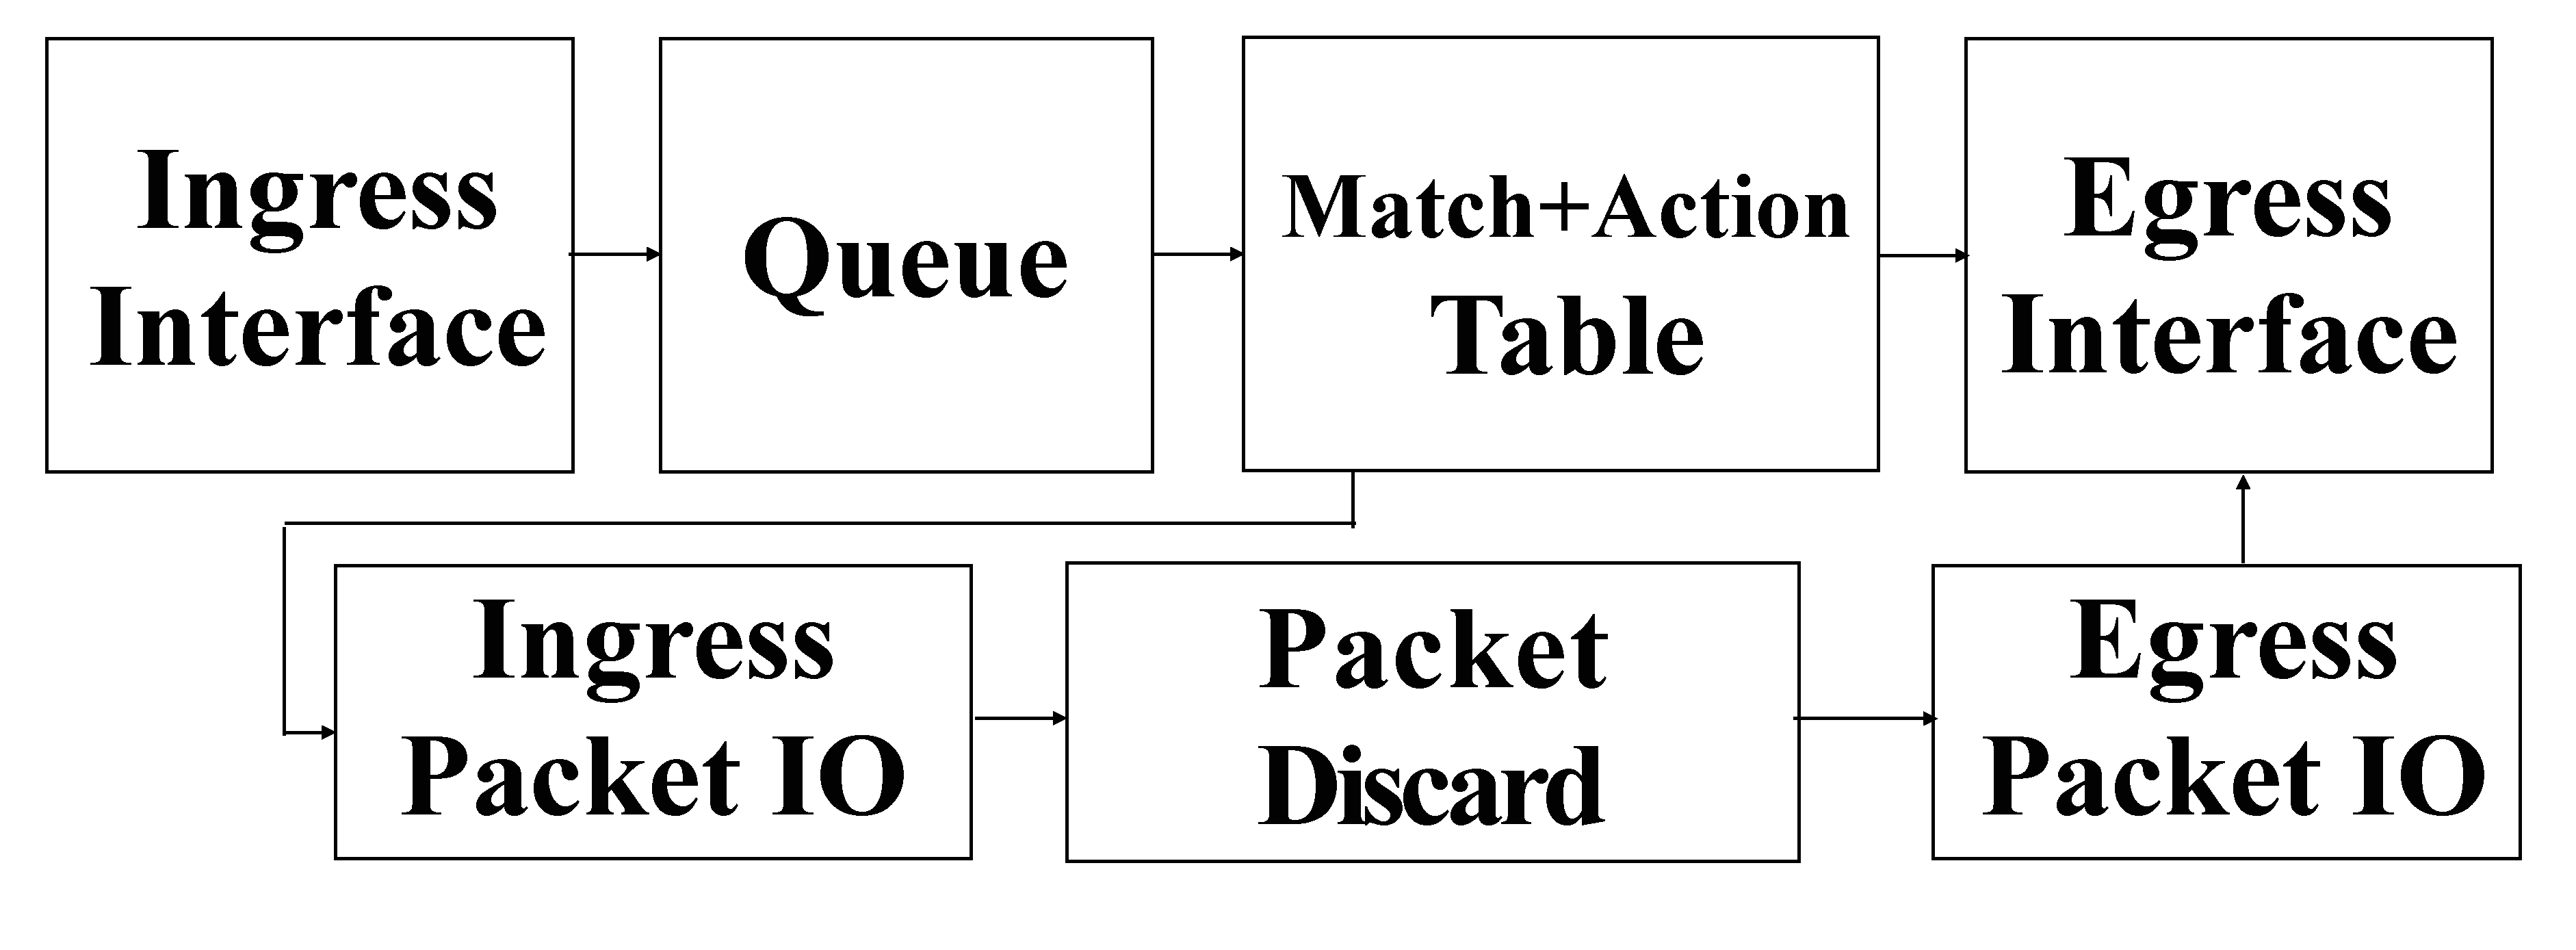
\includegraphics[width=.24\textwidth]{fig/MANE_1.eps}
    \caption{Packet processing in a P4-based MANE.}
    \label{MANE}
\end{figure}

Fig. ~\ref{MANE} shows how the P4-based MANE process packets. We define some header format and parsers which allow us to understand the structure of the packet. Incoming packets will first be parsed and divide into header and payload. We can design some match+action table in both ingress and egress control program to determine how to process the packet. In the ingress program, we can specify some match+action table to apply and may drop the packet if it's not valid or useless. After the packet pass the ingress program, it will be pushed into queues and than processed by the egress program. In P4, we can also calculate the checksum, configure forwarding table, construct some metadata adding to the header. With these tools and the knowledge of the whole Internet,  we can drop packets optimally in P4-based MANEs. 

On the other hand, P4-based MANE can not detect the condition of the whole Internet. Therefore, we combine P4-based MANE and SDN controller. Here we select {\em Open Network Operating System (ONOS)} to be our controller because it can from a controller plane without too many settings and it supports P4-runtime. P4-runtime is a program for controller to reconfig the P4-based MANEs. In other words, we can change the behavior of the P4-based MANE in runtime through P4-runtime. It works like a RESTful API server, we can simply give some commands to control our P4-based MANEs. 
\section{Tentative Solution} \label{sec:Tentive Soution}

To drop scalable video packets to retain streamed video quality when bandwidth is in sufficient and dynamic. We plan to implement the following three drop logics. (i) Tail, (ii) Enhancement Layer (EL), and (iii) Rate-Distortion Optimize (RDO). Tail always drop the last packet while EL drops the enhancement layer packets.  The advantage of tail is the simplicity. EL ensure the decodability since we always forward the base layer packet. RDO takes the nature of rates between packet length and distortion into consideration, and than drop the packet with largest rate. Furthermore, we will record the frame number and layer id of the dropped packet. Therefore, we can also drop the other packets with the same frame number and higher layer id. RDO logic aims to minimize the negative impact of dropping packets. 

\begin{figure}[tbh]
    \centering
    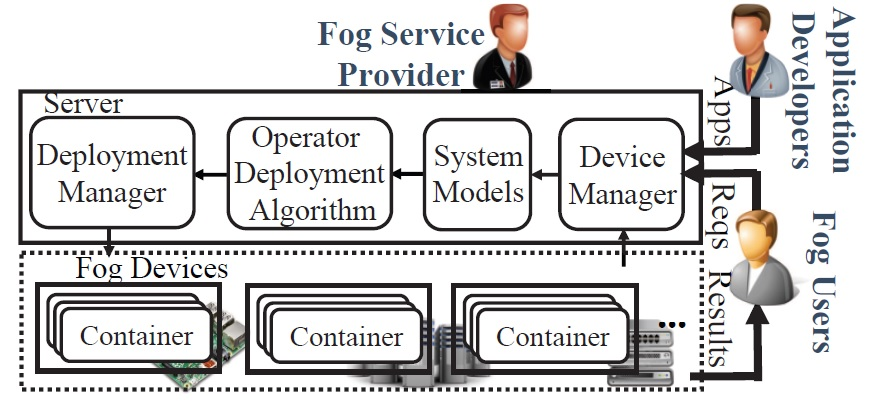
\includegraphics[width=0.40\textwidth]{fig/architecture.eps}
    \caption{High-level system architecture with a network of MANEs.}
\vspace{-0.1cm}
    \label{architecture} 
\end{figure}

Figure. ~\ref{architecture} show our architecture of the whole system. It is composed of a sender, some clients, some P4-based MANEs, some regular switches, and a ONOS controller connects those MANEs. The ONOS controller forms a control plane disassociate from the data plane. 

\section{Expect Outcome} \label{sec:Expect Outcome}


\section{Plan} \label{sec:Plan}

To approach our goal, we have learned how to write P4 programming language and setup our testbed inside Mininet. The next step is to finish our three drop logics, tail, EL, and RDO in our P4-based MANEs. Then we will run some experiments to make sure we optimally drop the packets. To leverage the advantage of SDN, we connect the P4-based MANEs with the ONOS controller. Next we will set up an server or write a program for developers to command our P4-based MANE in runtime, and we also need to make the controller able to reroute the flows if there's a physical disconnection.

%\section*{Acknowledgements}
%This work was partially supported by the Ministry of Science and Technology of Taiwan under the grant \#106-2221-E-007-101.
%\begin{figure}
%	\centering
%	\includegraphics[width=0.7\linewidth]{noms18Demo}
%	\caption{}
%	\label{fig:noms18demo}
%\end{figure}

%{\small
\bibliographystyle{abbrv}
\bibliography{./ref}
%}
\end{document}

